% --------------------------------------------------------------------------- %
% Poster for the ECCS 2011 Conference about Elementary Dynamic Networks.      %
% --------------------------------------------------------------------------- %
% Created with Brian Amberg's LaTeX Poster Template. Please refer for the     %
% attached README.md file for the details how to compile with `pdflatex`.     %
% --------------------------------------------------------------------------- %
% $LastChangedDate:: 2011-09-11 10:57:12 +0200 (V, 11 szept. 2011)          $ %
% $LastChangedRevision:: 128                                                $ %
% $LastChangedBy:: rlegendi                                                 $ %
% $Id:: poster.tex 128 2011-09-11 08:57:12Z rlegendi                        $ %
% --------------------------------------------------------------------------- %
\documentclass[a0paper,portrait]{baposter}

\usepackage{relsize}		% For \smaller
\usepackage{url}			% For \url
\usepackage{epstopdf}	% Included EPS files automatically converted to PDF to include with pdflatex
\usepackage{cite}
\usepackage{xcolor}

\usepackage{setspace}
\usepackage{amsmath}
\usepackage{mdwlist}
\usepackage{graphicx,stfloats}
\usepackage{booktabs}

\usepackage{siunitx}
\sisetup{per=slash, load=abbr}

\usepackage{calc}
\usepackage{array}
\usepackage{caption}
\usepackage{rotating}
\usepackage{url}
\usepackage{pgf,tikz}
\usepackage{pgfplots, pgfplotstable}
\usetikzlibrary{snakes,arrows,shapes}

\pgfplotsset{compat=newest}

%%% Global Settings %%%%%%%%%%%%%%%%%%%%%%%%%%%%%%%%%%%%%%%%%%%%%%%%%%%%%%%%%%%

\graphicspath{{pix/}}	% Root directory of the pictures 
\tracingstats=2			% Enabled LaTeX logging with conditionals

%%% Color Definitions %%%%%%%%%%%%%%%%%%%%%%%%%%%%%%%%%%%%%%%%%%%%%%%%%%%%%%%%%

\definecolor{bordercol}{RGB}{255,255,255}
\definecolor{headercol1}{RGB}{186,215,230}
\definecolor{headercol2}{RGB}{186,215,230}
\definecolor{headerfontcol}{RGB}{0,0,0}
\definecolor{boxcolor}{RGB}{255,255,255}
%\definecolor{boxcolor}{RGB}{186,215,230}

%%%%%%%%%%%%%%%%%%%%%%%%%%%%%%%%%%%%%%%%%%%%%%%%%%%%%%%%%%%%%%%%%%%%%%%%%%%%%%%%
%%% Utility functions %%%%%%%%%%%%%%%%%%%%%%%%%%%%%%%%%%%%%%%%%%%%%%%%%%%%%%%%%%

%%% Save space in lists. Use this after the opening of the list %%%%%%%%%%%%%%%%
\newcommand{\compresslist}{
	\setlength{\itemsep}{1pt}
	\setlength{\parskip}{0pt}
	\setlength{\parsep}{0pt}
}

%%%%%%%%%%%%%%%%%%%%%%%%%%%%%%%%%%%%%%%%%%%%%%%%%%%%%%%%%%%%%%%%%%%%%%%%%%%%%%%
%%% Document Start %%%%%%%%%%%%%%%%%%%%%%%%%%%%%%%%%%%%%%%%%%%%%%%%%%%%%%%%%%%%
%%%%%%%%%%%%%%%%%%%%%%%%%%%%%%%%%%%%%%%%%%%%%%%%%%%%%%%%%%%%%%%%%%%%%%%%%%%%%%%

\begin{document}
\typeout{Poster rendering started}

%%% Setting Background Image %%%%%%%%%%%%%%%%%%%%%%%%%%%%%%%%%%%%%%%%%%%%%%%%%%
\background{
	\begin{tikzpicture}[remember picture,overlay]%
	\draw (current page.north west)+(-2em,2em) node[anchor=north west]
	{};
	%{\includegraphics[height=1.1\textheight]{background}};
	\end{tikzpicture}
}

%%% General Poster Settings %%%%%%%%%%%%%%%%%%%%%%%%%%%%%%%%%%%%%%%%%%%%%%%%%%%
%%%%%% Eye Catcher, Title, Authors and University Images %%%%%%%%%%%%%%%%%%%%%%
\begin{poster}{
	grid=false,
	% Option is left on true though the eyecatcher is not used. The reason is
	% that we have a bit nicer looking title and author formatting in the headercol
	% this way
	%eyecatcher=false, 
	borderColor=bordercol,
	headerColorOne=headercol1,
	headerColorTwo=headercol2,
	headerFontColor=headerfontcol,
	% Only simple background color used, no shading, so boxColorTwo isn't necessary
	boxColorOne=boxcolor,
	headershape=roundedright,
	headerfont=\large\sf\bf,
	textborder=rectangle,
	background=user,
	headerborder=open,
  boxshade=plain
}
%%% Logo %%%%%%%%%%%%%%%%%%%%%%%%%%%%%%%%%%%%%%%%%%%%%%%%%%%%%%%%%%%%%%%%%%%%%%
{
	% The logos are compressed a bit into a simple box to make them smaller on the result
	% (Wasn't able to find any bigger of them.)
	\setlength\fboxsep{0pt}
	\setlength\fboxrule{0pt}
	\fbox{
		\begin{minipage}{15em}
			\includegraphics[width=15em]{logo}
		\end{minipage}
	}
	
}
%%%% Eye Cacther %%%%%%%%%%%%%%%%%%%%%%%%%%%%%%%%%%%%%%%%%%%%%%%%%%%%%%%%%%%%%%%
%{
%	Eye Catcher, empty if option eyecatcher=false - unused
%}
%%% Title %%%%%%%%%%%%%%%%%%%%%%%%%%%%%%%%%%%%%%%%%%%%%%%%%%%%%%%%%%%%%%%%%%%%%
{\huge\sf\bf
Hardware Acceleration Without The Use Of ~RTL
}
%%% Authors %%%%%%%%%%%%%%%%%%%%%%%%%%%%%%%%%%%%%%%%%%%%%%%%%%%%%%%%%%%%%%%%%%%
{
	\vspace{0.3em} Prashant Ravi\\
	{\smaller prashant014@ntu.edu.sg}
}



\headerbox{Background and Motivation}{name=problem,column=0,row=0}{
Major issues in mainstream adoption of FPGAs:
\begin{itemize}\itemsep1pt \parskip0pt
\item Difficulty of accelerator design at low level
\item Long compilation times (Place and route)
\item Poor design productivity
\end{itemize}
One possible solution is to use FPGA Overlay:
\begin{itemize}\itemsep1pt \parskip0pt
	\item Accelerator design in a high level language
	\item Fast compilation and development cycles	
	\item Easy to use even by novice programmers
	\item Puts the FPGA in the hands of software developers.	
\end{itemize}
Another solution is to use novel high level synthesis tools:
\begin{itemize}\itemsep1pt \parskip0pt
\item HLS tools to generate C to RTL, eg:Vivado HLS, SDSoC
\item OpenCL to hardware design synthesis eg:AOCL, SDAccel
\end{itemize}
}



\headerbox{Contributions}{name=scgra,column=0,below=problem}{
\begin{itemize}\itemsep1pt \parskip0pt
	\item Analysis of Overlay architectures like Vectorblox MXP and Altera OpenCL SDK as alternatives to pure RTL design flow. Highlighting the ease of use and fast learning curves of these methods.
	\item Benchmarking and comparison of timing performance as well as operations per cycle for the Vectorblox MXP processor and the Altera OpenCL Implementation with arm CPU implementation.
\end{itemize}


}



\headerbox{Observations}{name=analysis, column=0,below=scgra}{
The Vectorblox MXP soft vector processor:
\begin{itemize}\itemsep1pt \parskip0pt
	\item Extremely short learning curve
	\item The Vectorblox MXP C/C++ api is extremely easy to use.
	\item Full control of DMA and execution to programmer.
	\item Compilation and debugging time equal to that of traditional C/C++ debugging.
\end{itemize}
The Altera OpenCL SDK:
\begin{itemize}\itemsep1pt \parskip0pt
	\item Minimal modification of traditional OpenCL code required.
	\item kernel optimizations like vectorization, hardware replication for parallelism.
	\item Dynamic re-programming of FPGA at runtime with totally new kernel.
	\item Host code portability across all devices. 
\end{itemize}	
	

}



\headerbox{Conclusions and Future Work}{name=conclusion,column=0,below=analysis,above=bottom}{
\begin{itemize}\itemsep1pt \parskip0pt
	\item More popularity of overlays and high level synthesis tools.
	\item Place and route effeciency improvements in OpenCL to hardware.
	\item Overall generated hardware effeciency improvment.
	\item More awareness in the software world and amongst software developers.
\end{itemize}
} 



\headerbox{Efficient Overlay Architecture}{name=designmethod,column=1,row=0}{
2D array of tiles: 
\begin{itemize}\itemsep1pt \parskip0pt
	\item Programmable functional unit (FU) and routing resources in each tile
	\item Functional units interconnected via an island-style routing network
	\item Coarse grained switch boxes, connection boxes and routing channels as programmable routing resources
	\item Customizable channel width (CW), number of tracks in a routing channel%, for varying routability requirements% but at a higher area cost.	
\end{itemize}
%\vspace{-0.2em}
\setlength\fboxsep{0pt}
\setlength\fboxrule{0pt}
\begin{center}
\fcolorbox{white}{white!100}{
    \fbox{
        \begin{minipage}{19.4em}
        \begin{center}   
        \includegraphics[width=9.5em]{arch}   	
		\includegraphics[width=9.5em]{tile_new}
        \end{center}       	
        \end{minipage}
    }
}
\end{center}
}



\headerbox{DSP Block Based Functional Unit}{name=functionalunit,column=2,row=0}{
\begin{itemize}\itemsep1pt \parskip0pt
	\item Fully pipelined DSP48E1 as a programmable processing element (PE) 
	\item Achievable frequency near theoretical limits for providing high throughput
	\item A pre-adder, a multiplier and an ALU inside the functional unit
	\item Can support upto 3 operations 
	\item MUX based reordering logic to handle logical inequivalence at the PE inputs
	\item SRL based variable-length shift registers for balancing pipeline latencies	
\end{itemize}	
	%\vspace{-0.2em}
	\setlength\fboxsep{0pt}
	\setlength\fboxrule{0pt}
	\begin{center}
		\fcolorbox{white}{white!100}{
			\fbox{
				\begin{minipage}{19.4em}
					\begin{center}   
						\includegraphics[width=19.4em]{fu_new}
					\end{center}       	
				\end{minipage}
			}
		}
	\end{center}	
}

\headerbox{Rapid, Vendor-Independent, Automated Mapping of Compute Kernels}{name=setup,span=2,column=1,below=functionalunit}{
\begin{itemize}\itemsep1pt \parskip0pt
	\item C to DFG Transformation: DFG generation from a C description of the compute kernel
	\item DSP48E1 Aware Mapping: Compute node merging based on the capability of the DSP block
	\item Placement and Routing of FU Netlist: Using VPR for mapping nodes in the graph to the DSP blocks, and edges onto the coarse grained tracks
	\item Latency Balancing: Parsing VPR output files and generating a routing resource graph to determine the latency imbalance at each node and hence the required delays at the FU inputs
\end{itemize}	
\pgfdeclarelayer{background}
\pgfdeclarelayer{foreground}
\pgfsetlayers{background,main,foreground}

%\vspace{-0.2em}
%\setlength\fboxsep{0pt}
\setlength\fboxrule{0pt}
\begin{center}
	\fcolorbox{white}{white!100}{
		\fbox{
						\begin{minipage}{10em}
							\begin{center}      	
							\includegraphics[width=30em]{codesnip}	
		
							\end{center}
							
						\end{minipage}
			
		}
	}
\end{center}



}



\headerbox{Experimental Evaluation}{name=experiment1,span=2,column=1,below=setup,above=bottom}{
\begin{itemize}\itemsep1pt \parskip0pt
	\item Two example overlays on Zynq device to execute the benchmark set: a 5$\times$5 Overlay-I with CW=2 operating at 370 MHz and a 7$\times$7 Overlay-II with CW=4 operating at 300 MHz
	\item RTL generation of benchmarks using Vivado HLS for performance (throughput) comparison 
	\end{itemize}
\vspace{-2em}	

\setlength\fboxrule{0pt}
\begin{center}
	\fcolorbox{white}{white!100}{
		\fbox{



	\begin{minipage}{13em}
	\begin{center}      	
		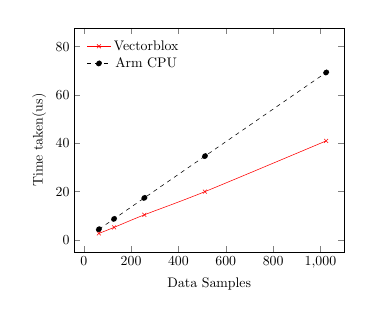
\begin{tikzpicture}[scale=0.5]
		\begin{axis}[
		xlabel=Data Samples,
		enlarge y limits = true,
		ylabel=Time taken(us),
		ymax = 80,
		xmax = 1100,
		legend pos=north west,
		legend style={draw=none}
		]
		\addplot [smooth,mark=x,red] plot coordinates {
			(64,     2.7)
			(128,    5.2)
			(256,    10.4)
			(512,    20)
			(1024,   41)			
		};
		\addplot [smooth,mark=*,dashed] plot coordinates {
			(64,     4.43)
			(128,    8.71)
			(256,    17.4)
			(512,    34.69)
			(1024,   69.30)
			
		};
		\legend{Vectorblox\\Arm CPU\\}
		\end{axis}
		\end{tikzpicture}
	\end{center}  
	\tiny  
	Vectorblox C API Implementation in Comparison with naive C Implementation on ARM CPU.
	\end{minipage}

	\hspace{1em}
	\begin{minipage}{13em}
	\begin{center}      				
	 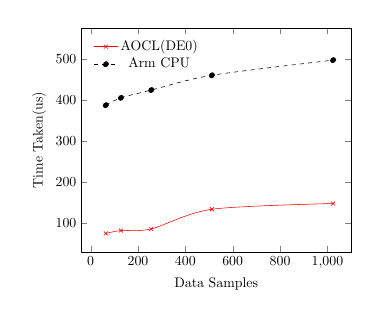
\begin{tikzpicture}[scale=0.5]
	 \begin{axis}[
	 xlabel=Data Samples,
	 ylabel=Time Taken(us),
	 enlarge y limits = true,
	 ymax = 530,
	 xmax = 1100,
	 legend pos=north west,
	 legend style={draw=none}
	 ]
	 \addplot [smooth,mark=x,red] plot coordinates {
			(64,     74)
			(128,    81)
			(256,    85)
			(512,    133)
			(1024,   147)			
		};
		\addplot [smooth,mark=*,dashed] plot coordinates {
			(64,     387)
			(128,    405)
			(256,    424)
			(512,    460)
			(1024,   497)
			
		};
	 \legend{AOCL(DE0)\\Arm CPU\\}
	 \end{axis}
	 \end{tikzpicture}
	\end{center}
	\tiny 
	OpenCL Implementation Timing Comparison between ARM CPU and AOCL FPGA Implementation.   					
	\end{minipage}
					
		}
	}
\end{center}



\vspace{-2em}	
%\vspace{-0.9em}
%\setlength\fboxsep{0pt}
\setlength\fboxrule{0pt}
\begin{center}
	\fcolorbox{white}{white!100}{
		\fbox{
			\begin{minipage}{38em}
				\begin{center}
					
					\tiny
					\begin{tabular}{@{}lc@{}r@{\phantom{x}}r@{\phantom{x}}r@{\phantom{x}}r@{}c@{}r@{\phantom{x}}r@{}c@{}r@{\phantom{x}}r@{\phantom{x}}r@{}c@{}r@{\phantom{x}}r@{\phantom{x}}r@{\phantom{x}}r@{\phantom{x}}r@{}}
						\toprule
						&\phantom{xx}&\multicolumn{4}{c}{Benchmark Characteristics}&\phantom{xx} 			&\multicolumn{2}{c}{Routability} 	&\phantom{xx}&\multicolumn{3}{c}{Overlay Results}	&\phantom{xx}	&\multicolumn{5}{c}{HLS Implementation Results}				\\
						\cline{3-6} \cline{8-9} \cline{11-13} \cline{15-19}
						Benchmark	&& i/o 		& op		& merged		& savings		&& CW=2					& CW=4 							&& Latency	& MLI 	& \textbf{GOPS}					    && Latency	& Fmax 	& \textbf{GOPS}		& Slices	& DSPs		    \\
									&& nodes	& nodes		& nodes			& 				&& 						&  								&& 			& 	 	& 						   			&& 			& 	 	& 			& 			& 			    \\
						\midrule
						chebyshev && 1/1		& 7			& 5				& 28\%			&& 3$\times$3			& 3$\times$3					&& 49		& 36	& \textbf{2.59}						&& 13		& 333	& \textbf{2.3}		& 24		& 3 		\\
						
						sgfilter  && 2/1		& 18		& 10			& 44\%			&& 4$\times$4			& 4$\times$4					&& 54		& 31	& \textbf{6.66}						&& 11		& 278	& \textbf{5.0}		& 40		& 8 		\\
						
						mibench   && 3/1		& 13		& 6				& 53\%			&& 3$\times$3			& 3$\times$3					&& 47		& 35	& \textbf{4.81}						&& 9 		& 295	& \textbf{3.8} 		& 81		& 3 		\\
						
						qspline   && 7/1		& 26		& 22			& 15\%			&& 5$\times$5			& 5$\times$5					&& 76		& 64	& \textbf{9.62}						&& 21		& 244	& \textbf{6.3}		& 126		& 14		\\
						
						poly1     && 2/1		& 9			& 6				& 33\%			&& 3$\times$3			& 3$\times$3					&& 34	 	& 22	& \textbf{3.33}						&& 12	 	& 285	& \textbf{2.56}		& 62		& 4			\\
						
						poly2     && 2/1		& 9			& 6				& 33\%			&& 3$\times$3			& 3$\times$3					&& 29		& 7		& \textbf{3.33}						&& 11		& 295	& \textbf{2.65}		& 45		& 4			\\
						
						poly3     && 6/1		& 11		& 7				& 36\%			&& 3$\times$3			& 3$\times$3					&& 31		& 11	& \textbf{4.07}						&& 12		& 250	& \textbf{2.75}		& 52		& 6			\\
						
						poly4     && 5/1		& 6			& 3				& 50\%			&& 2$\times$2			& 2$\times$2					&& 24		& 12	& \textbf{2.22}						&& 7		& 312	& \textbf{1.87}		& 36		& 3			\\
						
						atax      && 12/3		& 60		& 36			& 40\%			&& ---					& 6$\times$6					&& 72		& 58	& \textbf{18.0}						&& 13		& 263	& \textbf{15.8}		& 78		& 18		\\
						
						bicg      && 15/6		& 30		& 18			& 40\%			&& ---					& 6$\times$6					&& 46	 	& 32	& \textbf{9.0}						&& 7 	 	& 270	& \textbf{8.1} 		& 91 		& 18		\\
						
						trmm      && 18/9		& 54		& 36			& 33\%			&& ---					& 7$\times$7					&& 58		& 30	& \textbf{16.2}						&& 8 		& 222	& \textbf{11.9} 		& 105		& 36		\\
						
						syrk      && 18/9		& 72		& 45			& 37\%			&& ---					& 7$\times$7					&& 41		& 19	& \textbf{21.6}						&& 10		& 250	& \textbf{18}		& 237		& 24		\\
						\bottomrule
					\end{tabular}
					
					
				\end{center}
			\end{minipage}
		}
	}
\end{center} 	
}


\end{poster}
\end{document}
